% GNUPLOT: LaTeX picture with Postscript
\documentclass{minimal}
% Set font size
\makeatletter
\def\@ptsize{2}
\InputIfFileExists{size12.clo}{}{%
   \GenericError{(gnuplot) \space\space\space\@spaces}{%
      Gnuplot Error: File `size12.clo' not found! Could not set font size%
   }{See the gnuplot documentation for explanation.%
   }{For using a font size a file `size<fontsize>.clo' has to exist.
        Falling back ^^Jto default fontsize 10pt.}%
  \def\@ptsize{0}
  \input{size10.clo}%
}%
\makeatother
\renewcommand*\rmdefault{tm}%
% Load packages
\usepackage{graphicx}
\usepackage{color}
\makeatletter
% Select an appropriate default driver (from TeXLive graphics.cfg)
\begingroup
  \chardef\x=0 %
  % check pdfTeX
  \@ifundefined{pdfoutput}{}{%
    \ifcase\pdfoutput
    \else
      \chardef\x=1 %
    \fi
  }%
  % check VTeX
  \@ifundefined{OpMode}{}{%
    \chardef\x=2 %
  }%
\expandafter\endgroup
\ifcase\x
  % default case
  \PassOptionsToPackage{dvips}{geometry}
\or
  % pdfTeX is running in pdf mode
  \PassOptionsToPackage{pdftex}{geometry}
\else
  % VTeX is running
  \PassOptionsToPackage{vtex}{geometry}
\fi
\makeatother
% Set papersize
\usepackage[papersize={368.50bp,311.80bp},text={368.50bp,311.80bp}]{geometry}
% No page numbers and no paragraph indentation
\pagestyle{empty}
\setlength{\parindent}{0bp}%
% Load configuration file
\InputIfFileExists{gnuplot.cfg}{%
  \typeout{Using configuration file gnuplot.cfg}%
}{%
 \typeout{No configuration file gnuplot.cfg found.}%
}%
\usepackage[T1]{fontenc}
\usepackage{cmbright}
\usepackage{fancybox}
\usepackage{color}
\renewcommand{\familydefault}{\sfdefault}
\usepackage{bm}
\begin{document}
\begingroup
  \makeatletter
  \providecommand\color[2][]{%
    \GenericError{(gnuplot) \space\space\space\@spaces}{%
      Package color not loaded in conjunction with
      terminal option `colourtext'%
    }{See the gnuplot documentation for explanation.%
    }{Either use 'blacktext' in gnuplot or load the package
      color.sty in LaTeX.}%
    \renewcommand\color[2][]{}%
  }%
  \providecommand\includegraphics[2][]{%
    \GenericError{(gnuplot) \space\space\space\@spaces}{%
      Package graphicx or graphics not loaded%
    }{See the gnuplot documentation for explanation.%
    }{The gnuplot epslatex terminal needs graphicx.sty or graphics.sty.}%
    \renewcommand\includegraphics[2][]{}%
  }%
  \providecommand\rotatebox[2]{#2}%
  \@ifundefined{ifGPcolor}{%
    \newif\ifGPcolor
    \GPcolortrue
  }{}%
  \@ifundefined{ifGPblacktext}{%
    \newif\ifGPblacktext
    \GPblacktexttrue
  }{}%
  % define a \g@addto@macro without @ in the name:
  \let\gplgaddtomacro\g@addto@macro
  % define empty templates for all commands taking text:
  \gdef\gplbacktext{}%
  \gdef\gplfronttext{}%
  \makeatother
  \ifGPblacktext
    % no textcolor at all
    \def\colorrgb#1{}%
    \def\colorgray#1{}%
  \else
    % gray or color?
    \ifGPcolor
      \def\colorrgb#1{\color[rgb]{#1}}%
      \def\colorgray#1{\color[gray]{#1}}%
      \expandafter\def\csname LTw\endcsname{\color{white}}%
      \expandafter\def\csname LTb\endcsname{\color{black}}%
      \expandafter\def\csname LTa\endcsname{\color{black}}%
      \expandafter\def\csname LT0\endcsname{\color[rgb]{1,0,0}}%
      \expandafter\def\csname LT1\endcsname{\color[rgb]{0,1,0}}%
      \expandafter\def\csname LT2\endcsname{\color[rgb]{0,0,1}}%
      \expandafter\def\csname LT3\endcsname{\color[rgb]{1,0,1}}%
      \expandafter\def\csname LT4\endcsname{\color[rgb]{0,1,1}}%
      \expandafter\def\csname LT5\endcsname{\color[rgb]{1,1,0}}%
      \expandafter\def\csname LT6\endcsname{\color[rgb]{0,0,0}}%
      \expandafter\def\csname LT7\endcsname{\color[rgb]{1,0.3,0}}%
      \expandafter\def\csname LT8\endcsname{\color[rgb]{0.5,0.5,0.5}}%
    \else
      % gray
      \def\colorrgb#1{\color{black}}%
      \def\colorgray#1{\color[gray]{#1}}%
      \expandafter\def\csname LTw\endcsname{\color{white}}%
      \expandafter\def\csname LTb\endcsname{\color{black}}%
      \expandafter\def\csname LTa\endcsname{\color{black}}%
      \expandafter\def\csname LT0\endcsname{\color{black}}%
      \expandafter\def\csname LT1\endcsname{\color{black}}%
      \expandafter\def\csname LT2\endcsname{\color{black}}%
      \expandafter\def\csname LT3\endcsname{\color{black}}%
      \expandafter\def\csname LT4\endcsname{\color{black}}%
      \expandafter\def\csname LT5\endcsname{\color{black}}%
      \expandafter\def\csname LT6\endcsname{\color{black}}%
      \expandafter\def\csname LT7\endcsname{\color{black}}%
      \expandafter\def\csname LT8\endcsname{\color{black}}%
    \fi
  \fi
  \setlength{\unitlength}{0.0500bp}%
  \begin{picture}(7370.00,6236.00)%
    \gplgaddtomacro\gplbacktext{%
      \colorrgb{0.40,0.40,0.40}%
      \put(2016,2163){\makebox(0,0)[r]{\strut{} 0.01}}%
      \colorrgb{0.40,0.40,0.40}%
      \put(2016,2601){\makebox(0,0)[r]{\strut{} 0.1}}%
      \colorrgb{0.40,0.40,0.40}%
      \put(2016,3039){\makebox(0,0)[r]{\strut{} 1}}%
      \colorrgb{0.40,0.40,0.40}%
      \put(2016,3477){\makebox(0,0)[r]{\strut{} 10}}%
      \colorrgb{0.40,0.40,0.40}%
      \put(2016,3915){\makebox(0,0)[r]{\strut{} 100}}%
      \colorrgb{0.40,0.40,0.40}%
      \put(2016,4353){\makebox(0,0)[r]{\strut{} 1000}}%
      \colorrgb{0.40,0.40,0.40}%
      \put(2468,1923){\makebox(0,0){\strut{}2}}%
      \colorrgb{0.40,0.40,0.40}%
      \put(2776,1923){\makebox(0,0){\strut{}4}}%
      \colorrgb{0.40,0.40,0.40}%
      \put(3085,1923){\makebox(0,0){\strut{}6}}%
      \colorrgb{0.40,0.40,0.40}%
      \put(3393,1923){\makebox(0,0){\strut{}8}}%
      \colorrgb{0.40,0.40,0.40}%
      \put(3701,1923){\makebox(0,0){\strut{}10}}%
      \colorrgb{0.40,0.40,0.40}%
      \put(4009,1923){\makebox(0,0){\strut{}12}}%
      \colorrgb{0.40,0.40,0.40}%
      \put(4317,1923){\makebox(0,0){\strut{}14}}%
      \colorrgb{0.40,0.40,0.40}%
      \put(4626,1923){\makebox(0,0){\strut{}16}}%
      \colorrgb{0.40,0.40,0.40}%
      \put(4934,1923){\makebox(0,0){\strut{}18}}%
      \colorrgb{0.40,0.40,0.40}%
      \put(5242,1923){\makebox(0,0){\strut{}20}}%
      \colorrgb{0.40,0.40,0.40}%
      \put(5550,1923){\makebox(0,0){\strut{}22}}%
      \colorrgb{0.40,0.40,0.40}%
      \put(5858,1923){\makebox(0,0){\strut{}24}}%
      \colorrgb{0.40,0.40,0.40}%
      \put(6167,1923){\makebox(0,0){\strut{}26}}%
      \colorrgb{0.40,0.40,0.40}%
      \put(6475,1923){\makebox(0,0){\strut{}28}}%
      \colorrgb{0.40,0.40,0.40}%
      \put(6783,1923){\makebox(0,0){\strut{}30}}%
      \csname LTb\endcsname%
      \put(1234,3357){\rotatebox{-270}{\makebox(0,0){\strut{}$\delta Q^{[1]}/\delta Q^{[2]}$}}}%
      \put(4548,1563){\makebox(0,0){\strut{}Normal mode}}%
    }%
    \gplgaddtomacro\gplfronttext{%
    }%
    \gplbacktext
    \put(0,0){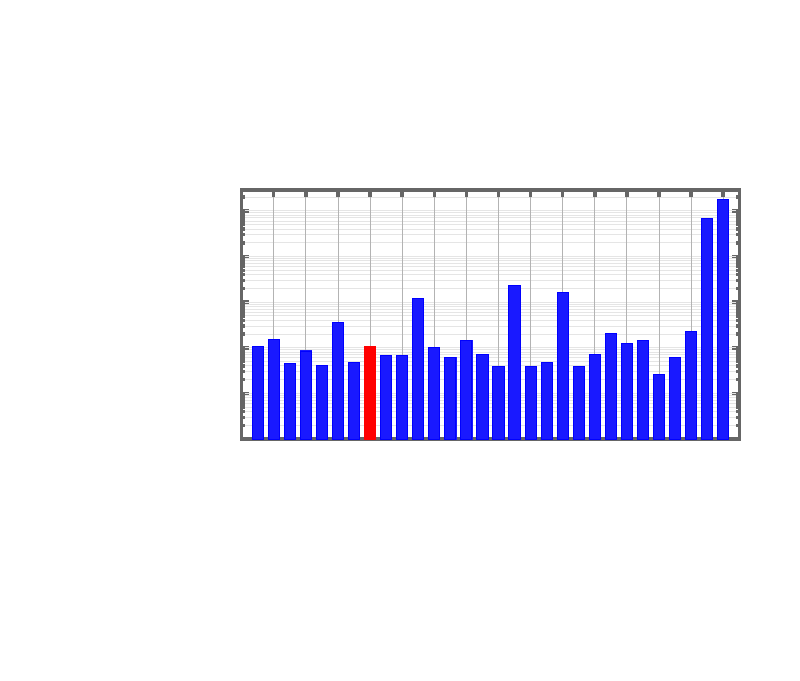
\includegraphics{nma-dq-inc}}%
    \gplfronttext
  \end{picture}%
\endgroup
\end{document}
